\documentclass[tikz,border=7mm]{standalone}
\usetikzlibrary{calc}
\begin{document}
  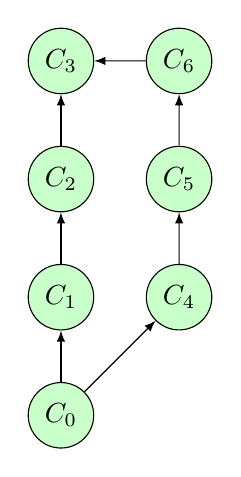
\begin{tikzpicture}[scale=1.5]
    \foreach \i in {0,...,6}
      \node[draw,circle,fill=green!21] (C\i) at ({div(\i,4)}, {div(\i,4)+mod(\i,4)}) {$C_\i$};
    \draw[-latex] foreach \i/\j in {0/1,1/2,2/3,0/4,4/5,5/6,6/3}{(C\i) edge (C\j)};
  \end{tikzpicture}
\end{document}
